%!TEX root = ../thesis.tex
%*******************************************************************************
%****************************** Second Chapter *********************************
%*******************************************************************************

\chapter{Related research}

% \ifpdf
%     \graphicspath{{Chapter2/Figs/Raster/}{Chapter2/Figs/PDF/}{Chapter2/Figs/}}
% \else
%     \graphicspath{{Chapter2/Figs/Vector/}{Chapter2/Figs/}}
% \fi


\section[Introduction]{Introduction}
Complex methods are often used in an attempt to rectify basic security aspects that should be prevalent in all authentication systems but are lacking. Biometric information remains unique to each individual and it is for that reason that it should be protected, and yet many developers neglect the importance of securing biometrics effectively. Due to this negligence, this research aims to present a novel approach for authentication systems to protect biometric information using a combination of transformation techniques and steganography encryption methods subsequent to the biometric information being captured by a leap motion controller. 

Within this chapter, an overview of the related topics will be given, followed by their current uses, implementations and relevance to this particular study. These topics include biometrics, cancelability, steganography and the use of a Leap Motion Controller peripheral device. Finally, the chapter will be concluded by coalescing the various techniques to provide theoretical proof of concept for the proposed authentication system.


\section[Biometrics]{Biometrics}
Biometrics have long been used as an accepted user authentication method and have been implemented as a security measure in many real-world systems including personal computers, mobile devices (cell phones and tablets), and also physical access control systems \citep{Shahim2016}.

Biometrics are the digitalisation and analysis of a person’s innate physical or biological characteristics and the use thereof to distinguish between persons that are to be afforded access to specific systems, information or physical areas \citep{Rathgeb2011}. By encoding a person’s physical attributes the disadvantages of traditional password based security, like passwords being lost or stolen, can be overcome \citep{Verma2016}. One of the factors that hampers the acceptance of biometric authentication systems is that the cost of the development and implementation has traditionally been high due to factors such as biometric hardware, computational processing power, infrastructure integration, user training, and research and testing (Verma \& Sinha, 2016). Furthermore, biometric systems present a unique challenge in terms of user privacy due to the personal nature of the biometric information that is stored in and used by the system \citep{Paul2012}.

The cost factor is one that decreases as continued development in the related hardware takes place. Alongside this development of dedicated biometric hardware there is an influx of new augmented computer interaction possibilities (i.e., new and non-traditional ways to control computers), a wide range of technological facets such as voice-, imaging- and movement control are receiving a lot of attention \citep{Paul2012, Verma2016}. Voice-control consists of verifying who the speaker is with the use of voice biometrics. This type of biometric has shown vast improvement recently and is often used to prove that low error-rates combined with high accuracy is achievable with its use. Image-control typically refers to facial recognition implementations, retina scanners and/or eye-tracking software that implement infrared imaging. In order to facilitate these interactions, the hardware is implicitly working with information that can be harnessed for biometric authentication. Hardware peripherals (like the leap motion controller (LMC)) that extend the basic functionality of computers to include support for voice and imaging facets are becoming more commonplace \citep{Rathgeb2011}. These peripherals are even used in biometrics research. For instance, \cite{Chan2015}, use an LMC for hand scanning and biometric authentication whereby a user would be able to gain access to a system, physical area or information by having their hand geometry scanned and analysed. They also posit the use of an LMC in multifactor authentication systems in combination with traditional passwords and PIN approaches. 
Typically, this type of biometric authentication process follows the protocol of matching prior biometric templates (i.e. digitally formatted biometric features) that are stored within a database to the biometrics that are presented to the system during the biometric scanning process. 

This study proposes a system that expands on the existing techniques for biometric authentication with an LMC. This expansion uses techniques from steganography to store binary representations of the biometrics within an image as a biometric template alternative. The system does not merely store the raw biometric data within the image, but rather applies transform parameters to it. Only once the transform parameters have been added to the original biometrics are they stored/matched to authenticate and authorise the user. This ensures that each users’ biometric information is neither compromised, nor exposed. 

Cancelable biometrics refers to protecting the biometric information from third party scrutiny by obfuscating this information. This addresses the challenge of privacy of biometric information as mentioned above and is further discussed in the next section.


\section[Cancelability]{Cancelability}
With the use of authentication systems becoming more prevalent, a primary concern becomes real-time processing of transmitted information as to verify a user’s identity. The authentication process itself within traditional systems has evolved and often resorts to biometric information rather than passwords, tokens and/or secret keys \citep{Verma2016}. This is primarily due to the inability of these traditional schemes to differentiate between an authentic user and an impostor. By authenticating users using biometric information the privacy of biometric data becomes important. Should attackers manage to gain access to the recognition system and its underlying data, the user-specific biometric information becomes readily available for identity theft. 
A possible solution would be to use multifactor biometric authentication with two or more biometric traits being employed. However, by adding more biometric features it will only add to the possible losses (should the system be compromised). Within the information security industry, one of the long acclaimed benefits of using biometric authentication has been that with post-enrolment biometric templates, user-specific biometric information (matching the stored template) could not be reconstructed. The benefit was refuted and once biometric templates become compromised, the biometric template is rendered useless \citep{Rathgeb2011}. This is because unlike passwords, biometric templates cannot simply be re-assigned due to their unique personal nature. Considering the susceptibility of such biometric authentication systems an approach to enhance the robustness can be used that is known as cancelable biometrics (CB). This approach improves upon standard encryption algorithms that expose biometric templates during the authentication attempt by not supporting the comparison of templates within the encrypted domain \citep{Rathgeb2011}. Simply put, the encrypted domain referred to by CB ensures that data will remain secure in transit and in storage. Furthermore, CB allows for re-issuing and/or regenerating biometric information with a unique and independent identity. The process of transforming or repeatedly distorting the biometric feature using transform parameters that are predetermined rather than using the original biometric achieves this \citep{Shahim2016}. As to meet some of the major requirements regarding biometric information protection, biometric cryptosystems (BCS) and CB are designed so that biometric features are \citep{Rathgeb2011, Verma2016}:

\begin{enumerate}[label=\roman*.]
	\item Diverse – Unable to be applied in multiple applications;
	\item Reusable – Reused/replaced in the event of compromise; and
	\item Irreversible – Computationally challenging to reconstruct the original biometric template, but simultaneously rudimentary to generate the protected biometric template.
\end{enumerate}

Various approaches may be adopted when considering an implementation schema for biometric systems. However, one must consider the alternatives to an approach as to ensure that the chosen method is feasible. Thus, both BCS and CB are presented in order to gain an objective understanding. 
BCSs are systems designed so that digital keys can be directly bound to a particular biometric \citep{Rathgeb2011}. One BCS approach is relevant to this particular study, namely biohashing which implements biometric key-generation. However, \cite{Rathgeb2011} state that an implementation should not exist that directly generates keys from biometric templates. They elaborate that biometric features cannot provide sufficient information to reliably obtain lengthy and renewable keys without relying on helper data. Helper data is public information that is used within the key generation/retrieval process in a BCS \citep{Rathgeb2011}.  This is useful to the study because helper data can be used to transform and obscure biometric information. Another approach to BCS is a biometric key-bind cryptosystem. This involves a secret key that relates to a biometric model by using helper data. To successfully implement this approach, facts regarding both the biometric model and the secret key may not be disclosed \citep{Eng2016}. According to \cite{Paul2014} and \cite{Rathgeb2011}, implementation of key-binding cryptosystems can occur through a "fuzzy" commitment and a fuzzy vault. The concept of fuzzy incorporates the generation of helper data extracted from biometric features using a secrecy key. The above-mentioned helper data, combined with the secrecy key are then both encrypted and stored in the database. In order to authenticate a user, the helper data then uses the model and biometric features to rebuild the key \citep{Eng2016}. A structural representation of this method can be seen below in Figure~\ref{fig:System structure for biometric authentication}.

% Figure - System structure for biometric authentication figure

\begin{figure}[htbp!] 
\centering    
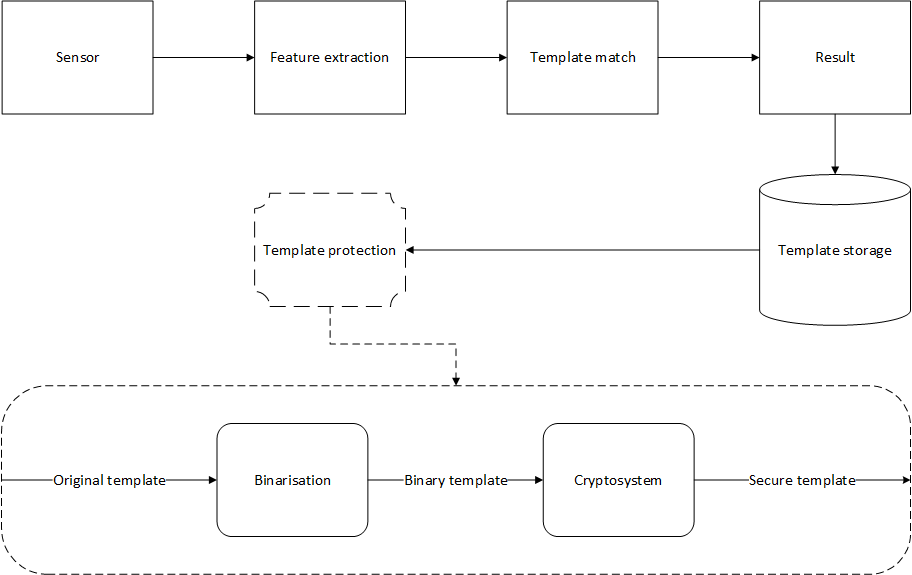
\includegraphics[width=1.0\textwidth]{Chapter2/Figs/Figure2-1.png}
\caption[System structure for biometric authentication]{System structure for biometric authentication}
\label{fig:System structure for biometric authentication}
\end{figure}

Initially, the sensor extracts the specific biometric features from the user (post-enrolment). Once the features have been extracted from the users, the current information within the system is then matched to that of the template that is stored within the database. However, during enrolment of the user in a BCS, the template that was created for each user undergoes a protection process that transforms the template into a secure template. The above-mentioned template protection process includes the binarisation of the extracted biometric features. Once the binary template is created, the template is then further processed by the cryptosystem to ultimately generate the secure template. This means that each time the user attempts to be authenticated, the extracted features use the helper data to rebuild the key and match the generated template to the secure template. Finally, if the templates match then the result will be positive and the user will gain access. 
Having considered a BCS, one needs to weigh up the options regarding the possible approaches to cancelability and implementations thereof. Cancelability, too, has the sole purpose of ensuring computational challenges when attempting to retrieve/recover the original biometric data by a third party (Rathgeb \& Uhl, 2011:1–25). The focal point regarding cancelability remains that biometric characteristics should remain innately robust so that even when transform parameters are applied the biometric features do not lose value/individuality. Along with individuality, by transforming biometrics one should ensure tolerance to intra-class variance so that the False Rejection Rate is not too high. Another important feature that cancelability has to offer is unlinkability \citep{Rathgeb2011}. This ensures that multiple transformed templates do not reveal any information relating to the original biometrics. In the unlikely event of data compromise, the transform parameters are simply altered which simultaneously implies biometric template updates. 
With regards to transforms within a CB implementation, two categories are forthcoming, namely \citep{Jain2016}:
  

\begin{enumerate}[label=\roman*.]
	\item Non-invertible transforms; and
	\item Biometric salting.
\end{enumerate}

The above-mentioned approaches differ in performance, accuracy and security. Depending on the system that is to be implemented, a weighted feasibility analysis should be conducted on those particular factors in order to select the most suitable approach. These approaches are briefly discussed below.

	\subsection{Non-invertible transforms}
	This approach involves the use of a non-invertible function that is applied to the biometric template. By applying this function, stored templates can be updated when transform parameters are modified \citep{Piciucco2016,Rathgeb2011}. Therefore, security is increased due to the inability to reconstruct the biometric data even though transforms may have been compromised. With this advantage comes an equal and opposite disadvantage. A loss of accuracy and a performance decrease is the disadvantageous result thereof. This is due to transformed biometric templates becoming laborious in comparison processing, which ultimately provides fewer biometric results to process during matching (thus, influencing the accuracy thereof).
	
	\subsection{Biometric salting}
	Biometric salting commonly involves biometric template transforms that are preferred invertible as opposed to the non-invertible approach (mentioned above). The term “salting” refers to the act of merging specific data (such as passwords) with unique random values (“salt”) in order to make all of the original data distinct \citep{SyedAhmad2012}. In this particular context, this technique may be applicable when a 4-digit PIN is used as the salt to be combined with the hand geometry vector prior to hashing the combination of data. This means that regardless of what biometric feature vector is chosen, the biometric template extraction cannot be reconstructed to the original biometric template \citep{Paul2014,Rathgeb2011}. This commands that transform parameters have to remain private. Variations of the approach may appear if user-specific transforms are applied \citep{teoh2008cancellable}. However, this demands that each authentication attempt requires transform parameters which may result in discrepancies if attackers successfully attain transform parameters. Ultimately, a decrease in performance is likely if the system implementation does not contain efficient biometric algorithms with high accuracy regarding private transform parameters. In contrast to non-invertible transforms, this approach maintains high recognition performance, however, the latter excels in terms of security \citep{Radha2011, Rathgeb2011}.



According to \cite{Rathgeb2011}, even though it is more common to adopt non-invertible approaches to system implementation schemes, biometric salting proves superior. Not only does biometric salting increase performance, but in user-specific transform applications by incorporating two-factor authentication one can improve both security and accuracy.

By taking a closer look at the general structure of using cancelable biometric it can be seen that during the enrolment phase, the features are extracted, transformed and then stored \citep{Patel2015}. This structure can be seen in the Figure~\ref{fig:Cancelable biometric system structure} below.

% Figure - Cancelable biometric system structure

\begin{figure}[htbp!] 
\centering    
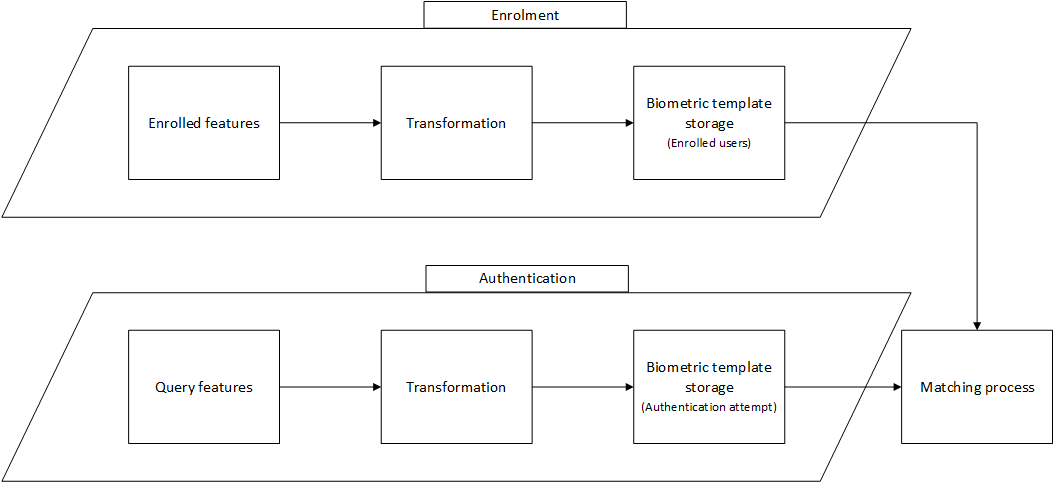
\includegraphics[width=1.0\textwidth]{Chapter2/Figs/Figure2-2.png}
\caption[Cancelable biometric system structure]{Cancelable biometric system structure}
\label{fig:Cancelable biometric system structure}
\end{figure}

The CB system structure is closely related to that of the BCS structure, however, the fundamental differences between the two are noticeable when attention is given to the timing of template protection. To argue these differences notice that in Figure~\ref{fig:System structure for biometric authentication} the template protection occurs post-storage, whereas, in Figure~\ref{fig:Cancelable biometric system structure} the template protection occurs after the feature extraction and prior to the storage during the transformation phase. Template protection is crucial within an authentication system with regards to attacks conducted upon the system. These template attacks will be further discussed below.

    \subsection{ Biometric template attacks}
    
    Conventional biometric systems have been subjected to numerous infiltration attacks that technologies such as BCS and CB appear to have been able to avert \citep{Rathgeb2011}. However, these techniques are known to have vulnerabilities. By analysing the structure of a generic biometric system, one is able to determine which particular processing points are vulnerable to attacks. The Figure~\ref{fig:Vulnerability points for biometric system attacks} below illustrates some of the above-mentioned vulnerabilities \citep{Patel2015}.
    
    % Figure - Vulnerability points for biometric system attacks
    
    \begin{figure}[htbp!] 
    \centering    
    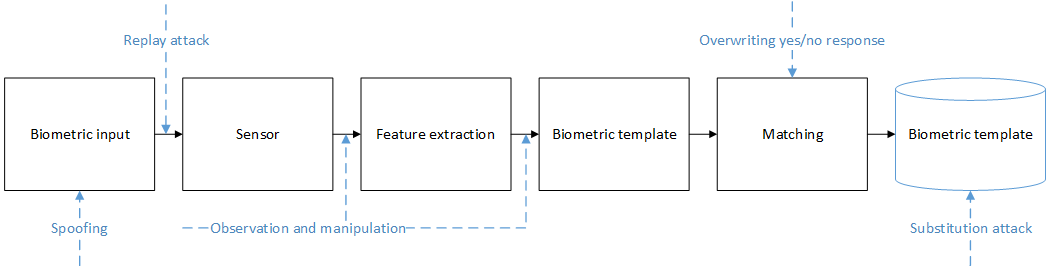
\includegraphics[width=1.0\textwidth]{Chapter2/Figs/Figure2-3.png}
    \caption[Vulnerability points for biometric system attacks]{Vulnerability points for biometric system attacks}
    \label{fig:Vulnerability points for biometric system attacks}
    \end{figure}
    
    Research shows that there are numerous vulnerable points to attack a generic biometric system \citep{Ratha2001}. However, an overview of the five points of attack mentioned above in Figure~\ref{fig:Vulnerability points for biometric system attacks} is presented as follows \citep{Karimovich2016, Patel2015, Ratha2001, Rathgeb2011}:
    
    \begin{enumerate}[label=\roman*.]
    
        \item Spoofing – This type of attack is implemented through the presentation of a   biometric to the biometric input (sensor). An example of this type of attack includes presenting a fake finger to the sensor and so forth.
        \item Replay attack – The use of this form of attack generally involves the resubmission of biometric data that is digitally stored which ultimately bypasses the biometric input device.
        \item Observation and manipulation – There are two entry points combined for this particular attack. The first entry point would attempt to attack the feature extractor with a Trojan horse in order to produce multiple feature sets that are specified by the attacker. The second entry point attempts to corrupt the manner in which the features are represented (with the assumption that the attacker is aware of the layout produced during feature extraction). Typically, the transition from extraction to matching is seamless, but should this process occur using the Internet, then this attack becomes a real concern.
        \item Overwriting yes/no response – The process of gaining access to the internal decision module and overwriting the final authentication decision. Also called a false acceptance attack.
        \item Substitution – Also referred to as a blended substitution attack. During this attack, the stored template is amalgamated with that of the attacker and used to authenticate.

    \end{enumerate}
    
    With the above-mentioned potential attacks in mind, the affected techniques and their potential attack formats should be classified. The attacks in correlation to BCS and CB can be seen in Table~\ref{table:Technique vulnerabilities} below.
    
    % Table - Technique vulnerabilities
    
    \begin{table}[h]
    \caption{Technique vulnerabilities}
    \centering
     \begin{tabular}{|p{0.45\textwidth} | p{0.45\textwidth}|} 
     \hline
    	\textbf{Potential attacks} & \textbf{Affected techniques(s)} \\ [1ex] 
     \hline\hline 
     Spoofing & BCS and CB  \\[1ex]
     \hline 
     Replay attack & BCS and CB \\[1ex]
     \hline
     Observation and manipulation & BCS and CB\\[1ex]
     \hline           
     Overwriting yes/no response & CB\\[1ex]
     \hline
     \end{tabular}
     \label{table:Technique vulnerabilities}
    \end{table}
    
    
    By considering both techniques and how each technique is vulnerable to diverse forms of attack, it is important to consider how to protect user biometrics against reconstruction. While analysis of template protection schemes are often rigorously analysed, the methods used for biometric feature transformation have not been the focal point of most approaches \citep{Nagar2009}. The protection of the user information throughout the use of information remains crucial to this particular system. 
    
    In an attempt to meet the requirement of non-invertible transforms, the use of a one-way hash algorithm could be applied to the transformed parameters as a final step prior to the matching process. The chosen algorithm standard will now be further discussed.

    \subsection{ Secure Hashing Algorithm}
    
    Cryptographic hash functions are designed to block malicious attempts of data modification \citep{Pfleeger2015}. The National Institute of Standards and Technology (NIST), as a part of the U.S. Department of Commerce, is responsible for publishing the Secure Hash Standard (SHS) and is implemented in an attempt to overcome various attacks. 
    
    The term Secure Hashing Algorithm (SHA) is used to describe the above-mentioned standard that can be further divided into four specific algorithms, namely SHA-0, -1, -2, and -3. The purpose of such an algorithm is to compute electronic data in a manner that produces a condensed representation of a message \citep{Foti2015}. The aforementioned representation is commonly known as a “message digest” or “hash.” The length of this message digest remains constant, regardless of the length of the original electronic input data. The algorithmic process that is followed (by all four algorithms as seen below) is one that is both iterative, as well as, unidirectional. By processing electronic data in such a manner, the algorithm ensures the integrity thereof. This is because in the event that the original data should be altered in the slightest, the resulting message digest will be completely contrasting to the message digest of the original data. 
    
    To liken the various versions of the SHA algorithms, a further analysis of each of the algorithms in terms of maximum input message size, block size, number of rounds executed and message digest size is presented. The SHA comparisons can be seen in Table~\ref{table: SHA comparisons}
    
    % Table - SHA comparisons
    
    \begin{table}[h]
    \caption{SHA comparisons}
    \centering
     \begin{tabular}{|p{0.18\textwidth} | p{0.18\textwidth}| p{0.18\textwidth}| p{0.18\textwidth}| p{0.18\textwidth}|} 
     \hline
    	\textbf{Algorithm} & \textbf{Maximum input message size (bits)} & \textbf{Block size(bits)} & \textbf{No. of rounds executed} & \textbf{Message digest size (bits)} \\ [1ex] 
     \hline\hline
     SHA-1 & \centering{$2$\textsuperscript{64}} & \centering{512} & \centering{80} & \centering{160} \tabularnewline 
     \hline
     SHA-2-224 & \centering{$2$\textsuperscript{64}} & \centering{512} & \centering{64} & \centering{224} \tabularnewline
     \hline
     SHA-2-256 & \centering{$2$\textsuperscript{64}} & \centering{512} & \centering{64} & \centering{256} \tabularnewline 
     \hline           
     SHA-2-384 & \centering{$2$\textsuperscript{128}} & \centering{1024} & \centering{80} & \centering{384} \tabularnewline
     \hline      
     SHA-2-512 & \centering{$2$\textsuperscript{128}} & \centering{1024} & \centering{80} & \centering{512} \tabularnewline 
     \hline
     SHA-3-256 & \centering{Unlimited} & \centering{1088} & \centering{24} & \centering{256} \tabularnewline
     \hline
     SHA-3-512 & \centering{Unlimited} & \centering{5761} & \centering{24} & \centering{512} \tabularnewline
     \hline
     \end{tabular}
     \label{table: SHA comparisons}
    \end{table}
    %TODO: Ref footnote
    It is important to note that prior to this study, the SHA-1 algorithm was broken by Google. A hash function is considered broken when two files happen to produce the same hash value (collision). The way in which this particular attack on SHA-1 occurred was through the use of a chosen-prefix attack. Google managed to use a precise piece of data that was injected into of the files. This caused the files to numerically align during the calculation process \citep{Stevens2017}.
    
    It was decided that SHA-2-256 would be further studied and implemented upon learning of the aforementioned collision and upon analysis of this table. Supplementary reasons for this choice include:
    
        \begin{enumerate}[label=\roman*.]
            
            \item SHA-2 has yet to be broken (unlike its predecessors);
            \item SHA-2-256 has a lower block size than those that follow; \item SHA-2-256 executes 64 rounds of hashing rather than 80; and
            \item A message digest of 256 bits is produced.

        \end{enumerate}
    
    Regardless of which SHA algorithm is chosen, the core functionality remains similar in the generation of unique hash values for any input that is fed into the algorithm. Each algorithm can be further divided into two phases, namely pre-processing and hash computations. To better explain the process followed within each of the two phases, see the Table~\ref{table: SHA phases} below \citep{Foti2015}.
    
    % Table - SHA phases
    
    \begin{table}[h]
        \caption{SHA phases}
        \begin{tabular}{|p{0.45\textwidth} | p{0.45\textwidth}|}
          \hline
         \textbf{Pre-processing} & \textbf{Hash computation} \\
         \hline\hline
            \begin{enumerate}
                \item Padding a message;
                \item Parsing the padded message into \newline \textit{m}-blocks; and
                \item Setting initialisation values for hash computation.
            \end{enumerate}
             & 
             \begin{enumerate}
                 \item Generates a message schedule from the padded message (along with functions, constants and word operations to iteratively generate a series of hash values; and
                 \item Uses the final hash value to determine the message digest.
             \end{enumerate} \\
             \hline
        \end{tabular}
        \label{table: SHA phases}
    \end{table}
    
    The entire SHA-2-256 algorithm can be summarised using the following set of equations.
    
    % SHA Equations 
    
    \begin{enumerate}
        
        \item \[W_t=\begin{cases}
                        M^{(i)}_t &, 0 \leq t \leq 15\\
                        ROTL[(W_{t-2}) + W_{t-7} + \sigma(W_{t-15}) + W_{t-16}  &], 16 \leq t \leq 63
                        \end{cases}\]
 
        
        \item Initialise the 8 working variables, \textit{a, b, c, d, e, f, g} and \textit{h}, containing hash values for (i-1): 
            \begin{gather*}     
                a = H^{(i-1)}_0, b = H^{(i-1)}_1, c = H^{(i-1)}_2, d = H^{(i-1)}_3, \\
                e = H^{(i-1)}_4, f = H^{(i-1)}_5, g = H^{(i-1)}_6, h = H^{(i-1)}_7 
            \end{gather*}
        \item For \textit{t} = 0 to 63:
            \begin{gather*}
                T_1 = h + \sum_{1}^{(256)}(e) + Ch(e,f,g) + K^{(256)}_t \\
                T_2 = \sum_{0}^{(256)}(a) + Maj(a,b,c) \\
                h = g, g = f, f = e, e = d + T_1, d = c, c = b, b = a \\
                a = T_1 + T_2 \\
            \end{gather*}
        
        \item Compute the intermediate hash values:
            \begin{gather*}
                H^{(i)}_0 = a + H^{(i-1)}_0, H^{(i)}_1 = b + H^{(i-1)}_1, H^{(i)}_2 = c + H^{(i-1)}_2, H^{(i)}_3 = d + H^{(i-1)}_3, \\ 
                H^{(i)}_4 = e + H^{(i-1)}_4, H^{(i)}_5 = f + H^{(i-1)}_5, H^{(i)}_6 = g + H^{(i-1)}_6, H^{(i)}_7 = h + H^{(i-1)}_7
            \end{gather*}
    \end{enumerate}
    
    To better explain the algorithm functionality, a use-case for this study will be presented using the SHA-2-256 algorithm in the form of a digital representation of hand measurements. These measurements can be summarised in text format as \textit{11, 12, 13, 14, 15}. Each number represents a transformed value for each of the five fingers.
    
    
        
        \subsubsection{ Pre-processing}
        First, each letter will be converted to binary. A one is added to the end to mark the end of the phrase. Next, get the phrase size. In this case, 112-bits. Eight bits per character makes it 112-bits and the rest get padded with zeros to get the block to the correct size. 
        
        \begin{enumerate}[label=\roman*.]
            
            \item 11, 12, 13, 14, 15 = 00110001 00110001 00101100 00110001 00110010 00101100 00110001 00110011 00101100 00110001 00110100 00101100 00110001 00110101 (112-bits);
            
            \item Add 1 to mark the end of the phrase;
            
            \item Pad the message with zeros (375-bits);
            
            \item Get the size of the phrase (11, 12, 13, 14, 15) = 24-bits.
            
        \end{enumerate}
        
        Upon completion of the four steps required for pre-processing, a block of 512 bits is formed and is presented in the Table~\ref{table:Pre-processing bit block example} below:
        \begin{table}[h]
            
            \caption{Pre-processing bit block example}
            \label{table:Pre-processing bit block example}
            \begin{center}
            \begin{tabular}{|c|}
             \hline     
             0011000100110001001011000011000100110010001011000011000100110011 \\
             001011000011000100110100001011000011000100110101\underline{1}000000000000000 \\
             0000000000000000000000000000000000000000000000000000000000000000 \\
             0000000000000000000000000000000000000000000000000000000000000000 \\
             0000000000000000000000000000000000000000000000000000000000000000 \\
             0000000000000000000000000000000000000000000000000000000000000000 \\
             0000000000000000000000000000000000000000000000000000000000000000 \\
             000000000000000000000000000000000000000000\textbf{1100010011000100110010} \\
             \hline
            \end{tabular}
            \end{center}
            
        \end{table}
        
        The message scheduler needs 64 words to be created from the block, but with each word being only 32-bits long, there is only enough for 16 words. 
        
        \begin{table}[h]
            \caption{Pre-processing bit block divided into 32 bit words}
            \centering
            \label{table:Pre-processing bit block divided into 32 bit words}
            
            \begin{tabular}{|c|}
            \hline  

            
              1. 00110001001100010010110000110001 \\
             
              2. 00110010001011000011000100110011 \\
             
              3. 00101100001100010011010000101100 \\
             
              4. 00110001001101011000000000000000 \\
             
              5. 00000000000000000000000000000000 \\
             
              6. 00000000000000000000000000000000 \\
             
              7. 00000000000000000000000000000000 \\
             
              8. 00000000000000000000000000000000 \\
             
              9. 00000000000000000000000000000000 \\
             
              10. 00000000000000000000000000000000 \\
             
              11. 00000000000000000000000000000000 \\
             
              12. 00000000000000000000000000000000 \\
             
              13. 00000000000000000000000000000000 \\
             
              14. 00000000000000000000000000000000 \\
             
              15. 00000000000000000000000000000000 \\
             
              16. 00000000001100010011000100110010 \\
             
            \hline
            \end{tabular}
        \end{table}
        
        
        Algorithm 2.1 formally describes how to create the other words. 
        % Equation for algorithm
        \begin{gather}
             \textbf{ROTL} [(W_{t-2}) + W_{t-7} + \sigma_0(W_{t-15}) + W_{t-16}]
        \end{gather}
        
        
        To get the 17th word, get the word 15 places back, in this case the second word, make 2 copies of it and right-rotate one of them by 7 places. This means each number moves one place to the right, 7 times, and when a number falls off the edge, it comes back on the other side. Right rotate the other by 18 places. Then right shift the last copy by 3. Right shift means that when a number falls off the edge, they are replaced with zeros on the other side. Do the same for the word 2 places back, 15th word, except right rotate by 17 and 19 places. Then right shift by 10. Add it to the word 16 places back, the 1st word and the words 7 places back, 10th word. Add all of these together and the 17th word generated. Proceed like this until there are 64 words. 
        
        \subsubsection{ Hash computation}
        
        The last part of the algorithm (step 3) uses the eight initial hash values and the 64 constant values. By converting between base 2 and base 16 is ultimately what produces the complex final signature. Table~\ref{table:Initial hashes and K-Constants} illustrates the aforementioned conversions with the final signature.
        
        
        % Table - Initial hashes and K-Constants
            
        \begin{table}[h]
        \caption{Initial hashes and K-Constants}
        \begin{tabular}{{|p{0.2\textwidth} | p{0.8\textwidth}|}}
          \hline
         \textbf{Initial hashes} & \textbf{K-Constants} \\
         \hline\hline
            \rule{0pt}{4ex}
                H(0) = a09e667  & 428a2f98 71374491 b5c0fbcf e9b5dba5 3956c25b 59f111f1 923f82a4 \\
                H(1) = b67ae85  & ab1c5ed5 d807aa98 12835b01 243185be 550c7dc3 72be5d74 80deb1fe \\
                H(2) = 3c6ef372 & 9bdc06a7 c19bf174 e49b69c1 efbe4786 0fc19dc6 240ca1cc 2de92c6f \\
                H(3) = a54ff53a & 4a7484aa 5cb0a9dc 76f988da 983e5152 a831c66d b00327c8 bf597fc7 \\
                H(4) = 510e527f & c6e00bf3 d5a79147 06ca6351 14292967 27b70a85 2e1b2138 4d2c6dfc \\
                H(5) = 9b05688c & 53380d13 650a7354 766a0abb 81c2c92e 92722c85 a2bfe8a1 a81a664b \\
                H(6) = 1f83d9ab & c24b8b70 c76c51a3 d192e819 d6990624 f40e3585 106aa070 19a4c116 \\
                H(7) = 5be0cd19 & 1e376c08 2748774c 34b0bcb5 391c0cb3 4ed8aa4a 5b9cca4f 682e6ff3 \\
                                & 748f82ee 78a5636f 84c87814 8cc70208 90befffa a4506ceb bef9a3f7 \\
                                & c67178f2 \\  
        \hline
        \end{tabular}
        \label{table:Initial hashes and K-Constants}
        \end{table}
       
        To get T1, use the value of \textit{e} and create three new words by right rotating by 6. 11 and 25. Then do an XOR on these values. Then run the Choose function of \textit{e, f} and \textit{g}. Get the first \textit{K} constant, the value of \textit{h} and the 1st word from the message scheduler and calculate the AND of all of these. 
        
        To get T2, run the Majority function over \textit{a, b} and \textit{c}. Then create 3 new words by right rotating \textit{a} by 2, 13 and 22. Then get the XOR of all of these and swap and modify the values as seen in the function.  
        
        This process is then repeated 64 times. 
        
        Lastly, AND the initial values for the hashes to the corresponding final values and concatenate them all together to produce the final message digest.
        
        % Equation 
        
        \begin{gather}
            H^{(N)}_0 || H^{(N)}_1 ||H^{(N)}_2 || H^{(N)}_3 || H^{(N)}_4 || H^{(N)}_5 || H^{(N)}_6 || H^{(N)}_7 
        \end{gather} 
        
        An example of a message digest can be seen when hand geometry measurements that have undergone transforms produce an initial output (prior to hashing) of: 

        \begin{center}
            \textbf{\textit{11, 12, 13, 14, 15}}
        \end{center}
        
        By using the SHA-1 hash algorithm, one sees a message digest (160 bits) of:
        
        \begin{center}
            \textbf{\textit{b4bf77f04af433a2ed748a44760f043acec04e35}}
        \end{center}
        
        With the same input string, using SHA-2-256 one sees a message digest (256 bits) of:
        
        \begin{center}
            \textbf{\textit{2c72ea316fc05ec89ede357ebe416fb80214396889462c07546978c18445310d}}
        \end{center}
        
    

Ultimately, this message digest would then be stored rather than the plaintext of the original data.

To conclude this subsection, the aim is to combine the key-binding capabilities of a BCS, the secure hashing algorithm and the biometric salting of CB. Once the user-specific biometric information has been transformed and is secure, it is ready for storage. In order to store this sensitive biometric information, rather than using a conventional database (due to its vulnerabilities, i.e. username/password exploits) a technique known as steganography was utilised and is described in the next section. 


\section[Steganography]{Steganography}
According to \cite{Kishor2016}, secret information is hidden using a type of communication, known as steganography. This is done through the use of multimedia files in conjunction with secret keys to embed information within these multimedia files. Steganography came about when it was realised that cryptography itself was incapable to securely transmit various forms of information across the Internet \citep{Jain2016}. The word steganography can be translated from Greek into “covered writing” \citep{Pandit2016}. When hiding sensitive information, the information in question is typically concealed using an alternative format to that of its original. This is done through regeneration of data using multimedia formats. Some of these formats include text, image, audio and even video. For the purposes of this particular study, focus will be maintained upon image steganography and the shrouding of sensitive biometric information by means of bit encryption within an image as the cover object. While cryptography disguises only the meaning of a message using code, steganography aims to hide the entire message from possible attackers \citep{Kishor2016, Pradhan2016}.

The conventional flow of image steganography (as seen in Figure~\ref{fig:Conventional image steganography flow}) follows a combination of encryption and decryption (just as cryptography does), but aims to use a confidential communication channel while secretly storing data and protecting the alteration of that data. An application that also makes this technique crucial to this particular study is the use of steganography as a conventional database alternative \citep{Pandit2016}.

% Figure - Conventional image steganography flow

  
\begin{figure}[htbp!] 
\centering    
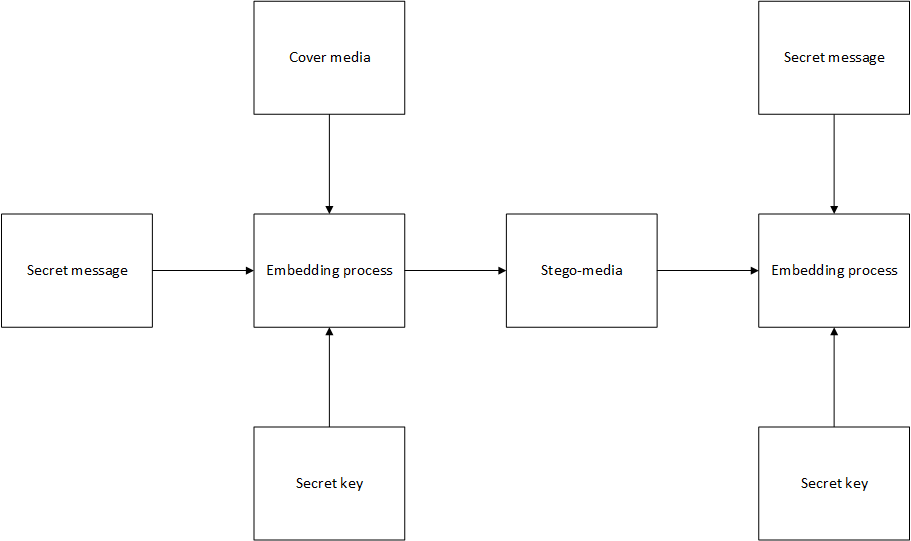
\includegraphics[width=1.0\textwidth]{Chapter2/Figs/Figure2-4.png}
\caption[Conventional image steganography flow]{Conventional image steganography flow}
\label{fig:Conventional image steganography flow}
\end{figure}

In image steganography, both the encryption process and the decryption process involve the use of a cover image and a stego-image. In short, the difference between the two is merely that the stego-image contains the sensitive information, while the cover image can be seen as an empty data storage location for the sensitive information. In Figure~\ref{fig:Conventional image steganography flow}, the steganography process requires sensitive information that is to be stored within the cover media (in this case, the image). This sensitive information is embedded into the image with the use of a secret key and a cover image to hide the information in. With the embedded information, the image is then referred to as the “stego-image.” The sensitive information can then only be extracted if the secret key is known.

Steganography can be implemented in various ways. However, the two major techniques that will be discussed regarding image steganography involve the following \citep{Pradhan2016, Paul2012}:

\begin{enumerate}[label=\roman*.]
	\item Spatial domain technique; and 
	\item Transform domain technique.
\end{enumerate}

The main difference between the two techniques is that when implementing a spatial domain steganography, the pixels within the image are directly manipulated. This is juxtaposed to the transform domain steganography that uses distinct transformations to allow image transformation in the transform domain and then only is the sensitive information stored with the image \citep{Pradhan2016, Roy2016}.

Literature broadens the scope of steganography even more in stating that spatial and transform domain techniques branch out into subcategories of implementation \citep{Radha2011, SyedAhmad2012, Verma2016}. A few examples of these methods can be seen in the Table~\ref{table: Steganography methods}.

\begin{table}[h]
\caption{Steganography methods}
\centering
 \begin{tabular}{|p{0.45\textwidth} | p{0.45\textwidth}|} 
 \hline
	\textbf{Spatial Domain} & \textbf{Transform Domain} \\ [1ex] 
 \hline\hline 
 Least Significant Bit substitution & Discrete Cosine Transform  \\[1ex]
 \hline 
 Pixel Value Differencing & Discrete Wavelet Transform  \\[1ex]
 \hline
 Random pixel selection & Discrete Fourier Transform  \\ [1ex] 
 \hline
 \end{tabular}
 \label{table: Steganography methods}
\end{table}


The purpose of modern steganography is to allow the host image protection so that the image itself, as well as the sensitive data it holds may not be recovered from the stego-image. By achieving this, the technique implemented is classified as irreversible steganography. The aforementioned objective is typically partnered with the ability to conceal sensitive information in a natural image in such a way that distortion of that image is minimal.

It is important to maintain that this particular study focusses on cancelable biometrics being stored using steganography techniques. This implies that, for the purposes of this research, the image may be distorted without it being an issue because even if an attacker manages to access the stego-image, he/she should not know what type of information is being stored, nor how to recover to biometrics after the transforms. 

According to \cite{Jain2016} and \cite{Pradhan2016}, steganography techniques are evaluated using various criteria. However, evaluation criteria that is relevant to this particular study are the following:

\begin{enumerate}[label=\roman*.]
	
	\item Hiding capacity – This is the maximum amount of data that can be stored within an image with reference to bits per pixel (bpp). Comparatively speaking, a larger hiding capacity means the steganography technique is better.
	
	\item Security Analysis – The technique should be able to withstand attacks to the image that include any attempt to alter the image.
	
	\item Robustness – By being robust against attempts to attack the image statistically, as well as image manipulation attacks, the technique alone provides protection to the sensitive information hidden within the image. 
	
	\item Computational complexity – With an algorithmic implementation, it is always important to take into consideration the time and space complexity.

\end{enumerate}
	
An image can be seen as a two-dimensional function, where the F(x, y) is the image pixels that can be represented as a grid. Each pixel contains ARGB (Alpha-Red-Green-Blue) values. Alpha values represent the pixel’s opacity and RGB values represent a particular colour within the colour system. These ARGB values range from (0, 0, 0, 0) to (255, 255, 255, 255). To embed data, one can either store information sequentially or randomly among various image pixels using the F(x, y) grid layout. By using sequential embedding of data one makes the data more susceptible to steganalysis detection by clustering the sensitive information within the image grid \citep{Laskar2013}. Randomly embedding data complicates the detection process by scattering the data using a random number sequence. The proposed system aims to use steganography techniques in the storage and obscuring of sensitive biometric information within a(n) image(s) once the biometric information has been transformed using CB techniques. In the next subsection, the means by which biometric information will be extracted using an LMC as the biometric scanner will be discussed.


\section[Leap motion controller ]{Leap motion controller }

With the LMC’s advanced hand and finger tracking capabilities, the position, velocity and orientation of all ten fingers, supplemented by hand geometry information, are reported upon with accuracy and low latency \citep{SyedAhmad2012}. \cite{Chan2015}  presented the implementation of an LMC to assume the role of a biometric authentication device by harnessing the above-mentioned information. The low-cost factor of this device makes this implementation even more favourable in situations where cost is of substantial concern. One drawback of this approach is that the LMC is a peripheral device that still requires a computer system to connect it to as the device cannot function in a stand-alone way. This disadvantage will add to the associated cost of implementation.

The LMC is able to scan a human hand at approximately 100 frames per second (FPS). With the use of an LMC it is possible to extract all finger/bone measurements of any given hand during an infrared scan. Any given combination of these measurements should be unique to every person \citep{Chan2015}. As seen in Figure~\ref{fig:Example_of_LMC_generated_hand_model}, a model of the hand is then created based on the readings taken by the LMC.

% Figure - Example of LMC generated hand model

  
\begin{figure}[htbp!] 
\centering    
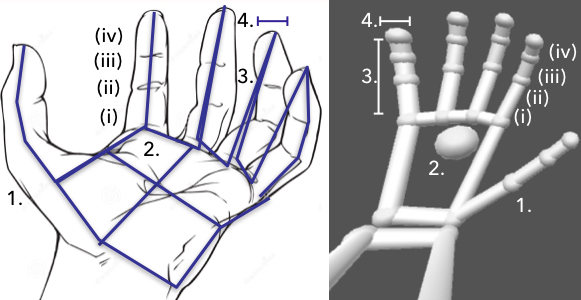
\includegraphics[width=1.0\textwidth]{Chapter2/Figs/Figure2-5.png}
\caption[Example of LMC generated hand model]{Example of LMC generated hand model}
\label{fig:Example_of_LMC_generated_hand_model}
\end{figure}

\begin{figure}
\centering
\def\svgwidth{\columnwidth}

\end{figure}



Information retrieved from the hand scans are summarised in Table~\ref{table: Relevant LMC readings}. The LMC is capable of acquiring numerous metrics relating to any presented hand. A combination of Figure~\ref{fig:Example_of_LMC_generated_hand_model} and Table~\ref{table: Relevant LMC readings} provides an overview of the metrics that are relevant to the proposed system. The measurements i-iv can be further explained as the acquired lengths and widths of each of these bones.

\begin{table}[h]
\caption{Relevant LMC readings}
\centering
 \begin{tabular}{|p{0.45\textwidth} | p{0.45\textwidth}|} 
 \hline
	\textbf{Readings} & \textbf{Bone} \\ [1ex] 
 \hline\hline 
 1.	Left/Right (Hand) & (i) Metacarpal \\[1ex]
 \hline 
 2.	Palm Width (Hand) & (ii) Proximal \\[1ex]
 \hline
 3.	Length (Fingers) & (iii) Intermediate \\ [1ex] 
 \hline
 4.	Width (Fingers) & (iv) Distal \\ [1ex] 
 \hline
 \end{tabular}
 \label{table: Relevant LMC readings}
\end{table}


All of the above information becomes relevant when attempting to authenticate users based on their hand-geometry. Although the LMC maintains great accuracy when gathering information regarding to the presented hand, the readings tend to differ depending on the position of the hand in relation to the LMC device itself. The readings show minimal discrepancy (see Chapter 4); however, this could become an issue when statistically analysing the false acceptance rate and false rejection rate of the final authentication system \citep{Nagar2009}.

While scanning the hand using an LMC one can vary the length of the scans to acquire a larger data set for each user reading during the enrolment and storage phase. This allows for the system to iterate through the hand and its 19 bones (three bones per finger, except for the intermediate bone which is non-existent in the thumb) within the fingers and retrieve the lengths of each of those bones.

With the use of an LMC, features can be extracted from presented hands, transformed to implement CB and stored using steganography techniques. A proposed framework to implement such a system is discussed in the following section.


\section[Chapter summary]{Chapter summary}

The aim of this chapter was to provide sufficient background and insight into the various techniques that are to be used throughout the implementation of the cancelable biometric authentication system. The concepts and techniques that were explained are used in the chapters that follow. Cancelable biometrics (along with the secure hashing standard), steganography and the use of the leap motion controller were explained with comparisons between different implementations thereof. This was done in order to select the best suited method that combines all the techniques in a manner that achieves secure storage of users’ hand geometry by using steganography.
Chapter 2 serves as a basis for the decision making process prior to the system implementation and offers the necessary literature to support the chosen techniques.


